\documentclass{beamer}
\usepackage{listings}
\usepackage{mdframed}
\usepackage{tikz}
\usepackage{pdfpages}
\usepackage[francais]{babel}
\usepackage[utf8]{inputenc}
\usepackage{float}
\usepackage{graphicx}
\usepackage{wrapfig}
\usepackage{times}
\usepackage[T1]{fontenc}
\usepackage[overlay,absolute]{textpos}

\newcommand{\firstlogo}{mdl.png}
\newcommand{\secondlogo}{ups.jpg}
\newcommand{\footsubject}{BandStorm, Le réseau social pour les amateurs de musique} 
\newcommand{\rgbcolortheme}{55,71,79}

\makeatletter
\hypersetup{pdfpagemode=FullScreen}

\mode<presentation> {
	\usepackage{../beamer-theme/beamerthemeUNLTheme}
}

\title[] % (facultatif, \`a utiliser uniquement si le titre de l'article est trop long)
{BandStorm, le réseau social pour les amateurs de musique}
\subtitle {IVVQ}

\newcommand{\authors}{%
Julian \bsc{Bironneau}\newline
Antoine de \bsc{Roquemaurel}\newline 
Steve \bsc{Magras}\newline
Dylan \bsc{Roletto}\newline
Zaccaria \bsc{Zyat}\newline
\newline~\newline{}\url{https://m2dl-bandstorm.herokuapp.com}
}
\newcommand{\JulianSpeak}{%
\author[
\textbf{\color{white}J}ulian\\
Antoine\\
Steve\\
Dylan\\
Zaccaria
]{\authors}
}

\newcommand{\NooneSpeak}{
\author[
Julian\\
Antoine\\
Steve\\
Dylan\\
Zaccaria
]{\authors}
}

\newcommand{\AntoineSpeak}{
\author[
Julian\\
\textbf{\color{white}A}ntoine\\
Steve\\
Dylan\\
Zaccaria
]{\authors}
}

\newcommand{\SteveSpeak}{
\author[
Julian\\
Antoine\\
\textbf{\color{white}S}teve\\
Dylan\\
Zaccaria
]{\authors}
}
\newcommand{\DylanSpeak}{
\author[
Julian\\
Antoine\\
Steve\\
\textbf{\color{white}D}ylan\\
Zaccaria
]{\authors}
}
\newcommand{\ZacSpeak}{
\author[
Julian\\
Antoine\\
Steve\\
Dylan\\
\textbf{\color{white}Z}accaria
]{\authors}
}


\institute[] 
{
Universit\'e Toulouse III -- Paul Sabatier \\
M1 Informatique -- Développement Logiciel 
\vspace{-10px}
}

\date[ ~ ~ ~ 13 / 11 / 2015] % (facultatif, peut être une abr\'eviation du nom de la conf\'erence)
{Vendredi 13 Novembre 2015}



\AtBeginSection[] {
\begin{frame}<beamer>{Plan}
	\tableofcontents[currentsection,subsectionstyle=hide]
\end{frame}
}

\setbeamerfont*{section in sidebar}{size=\fontsize{8px}{2.3em}\selectfont }
\setbeamerfont*{subsection in sidebar}{size=\fontsize{5px}{1.5em}\selectfont }
\begin{document}
	\sidetoc{no}
	\NooneSpeak{}
	\begin{frame}
		\titlepage
	\end{frame}

	\sidetoc{yes}
	\DylanSpeak
	\begin{frame}
		\tableofcontents[subsectionstyle=hide]
	\end{frame}
	\section{Gestion de projet} % Intro + Projet &=&  4'
	\DylanSpeak
\subsection{Présentation du projet}
\begin{frame}{Le projet BandStorm}
	\begin{itemize}
		\item Réseau social pour amateurs de musique
	\end{itemize}
	\vfill
	\begin{block}{Différentes fonctionnalités}
		\begin{itemize}
			\item Poster des statuts
			\item Suivre des utilisateurs
			\item Rejoindre des groupes
			\item Créer des événements
		\end{itemize}
	\end{block}
\end{frame}

\JulianSpeak
\subsection{Agilité}
\begin{frame}{Méthode Scrum}
\begin{figure}
\centering
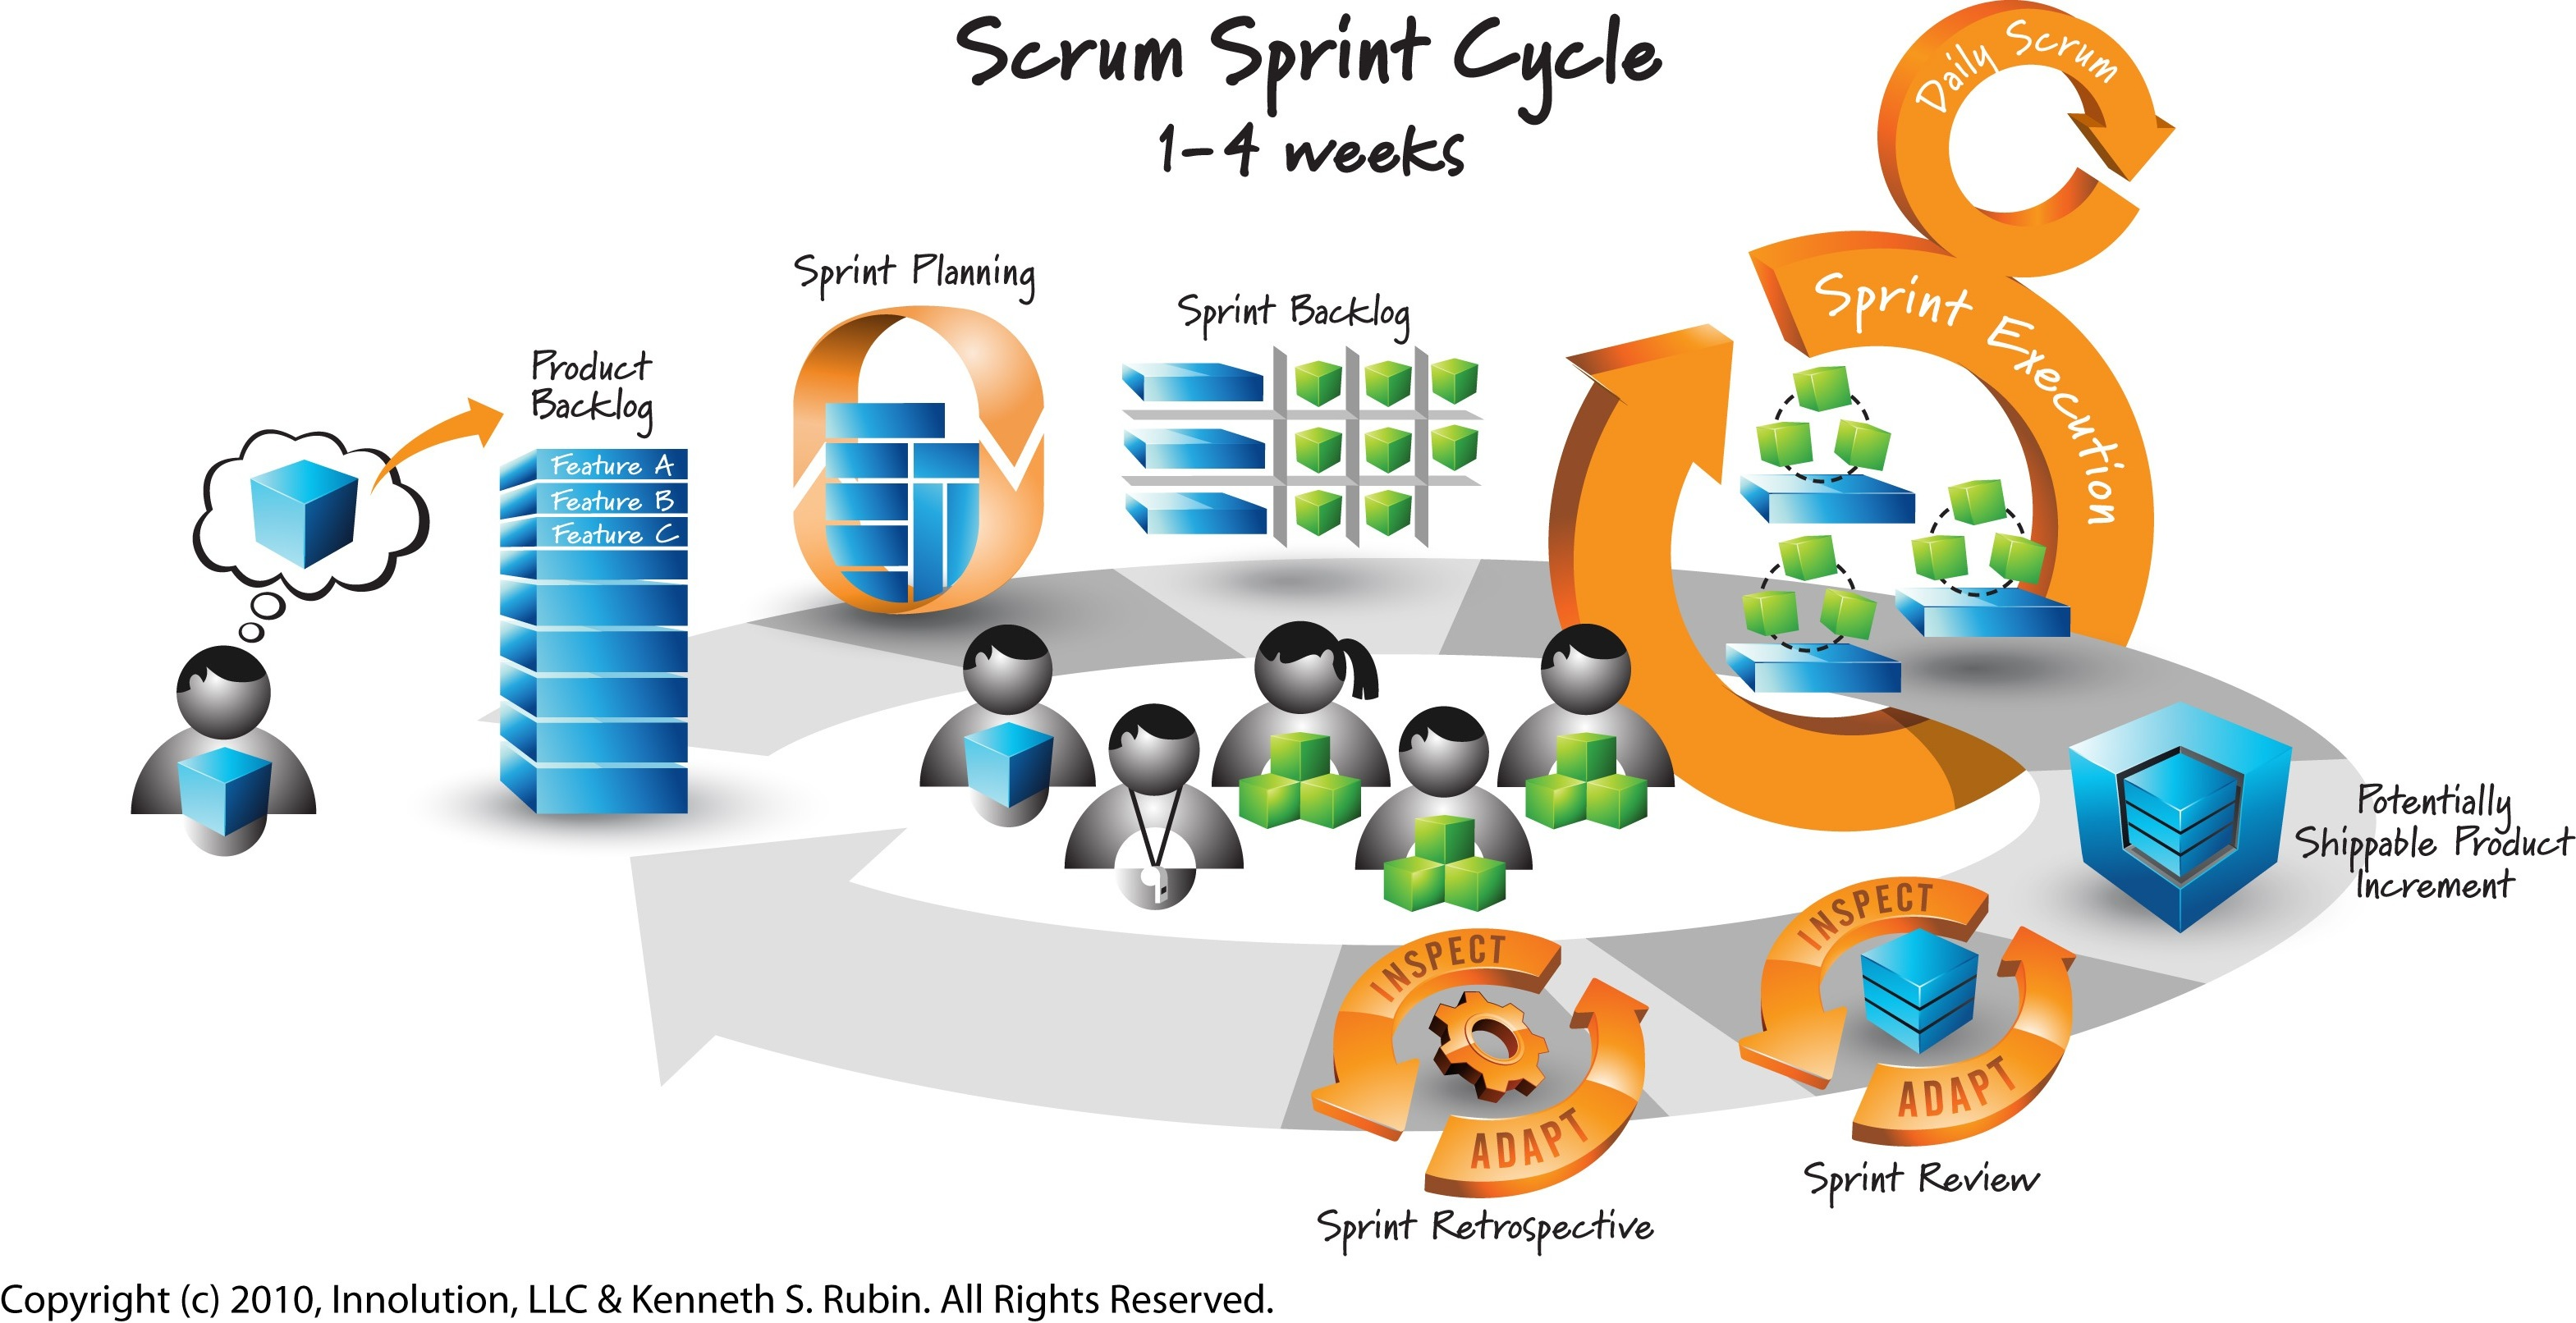
\includegraphics[width=\linewidth]{images/projectManagement/scrum}
\caption{Fonctionnement d'un Sprint avec Scrum}
\label{fig:scrum}
\end{figure}
\end{frame}

\begin{frame}{Définition de << fini >>}
	Une \textit{story} est finie si : 
	\vspace{-10px}
	\begin{itemize}
		\item Testée (unitaire et intégration)
		\item Couverture de tests en ligne \texttt{> 80\%}
%		\begin{itemize}
%			\item 100\% couverture (classes de modèles)
%			\item 80\% couverture (contrôleurs)
%			\item 80\% couverture (services)
%		\end{itemize}
		\item Test d'acceptance validé (\textit{Product Owner})
		\item Build Travis CI \textit{passed}
		\item Pas de majeurs \texttt{Codenarc}
		\item Pas de \textit{major} \& \textit{critical} \texttt{SonarQube}
		\item Javadoc rédigée
	\end{itemize}
	\vfill
	\pause
	Lors qu'une \textit{story} est terminée : 
	\vspace{-10px}
	\begin{itemize}
		\item Passage dans la colonne \textit{done}
		\item Fusion de la fonctionnalité dans la branche mère
	\end{itemize}
%		\item Branche pour l’issue GitHub
%		\item \textit{Pull request} revue (product owner)

%		\item 	Build Travis CI : OK
%		\item 	Codenarc : OK 
%		\item 	SonarQube : correction criticals & majors
%				\item Javadoc rédigée
%	Story → colonne “done”.
%	Fusion de la branche (story) dans la branche mère (Sprint).




\end{frame}

	\section{Processus de développement} %  Méthodo = 8'
	\AntoineSpeak
\subsection{Intégration}
\begin{frame}{Intégration\ldots}
\begin{figure}
	\centering
	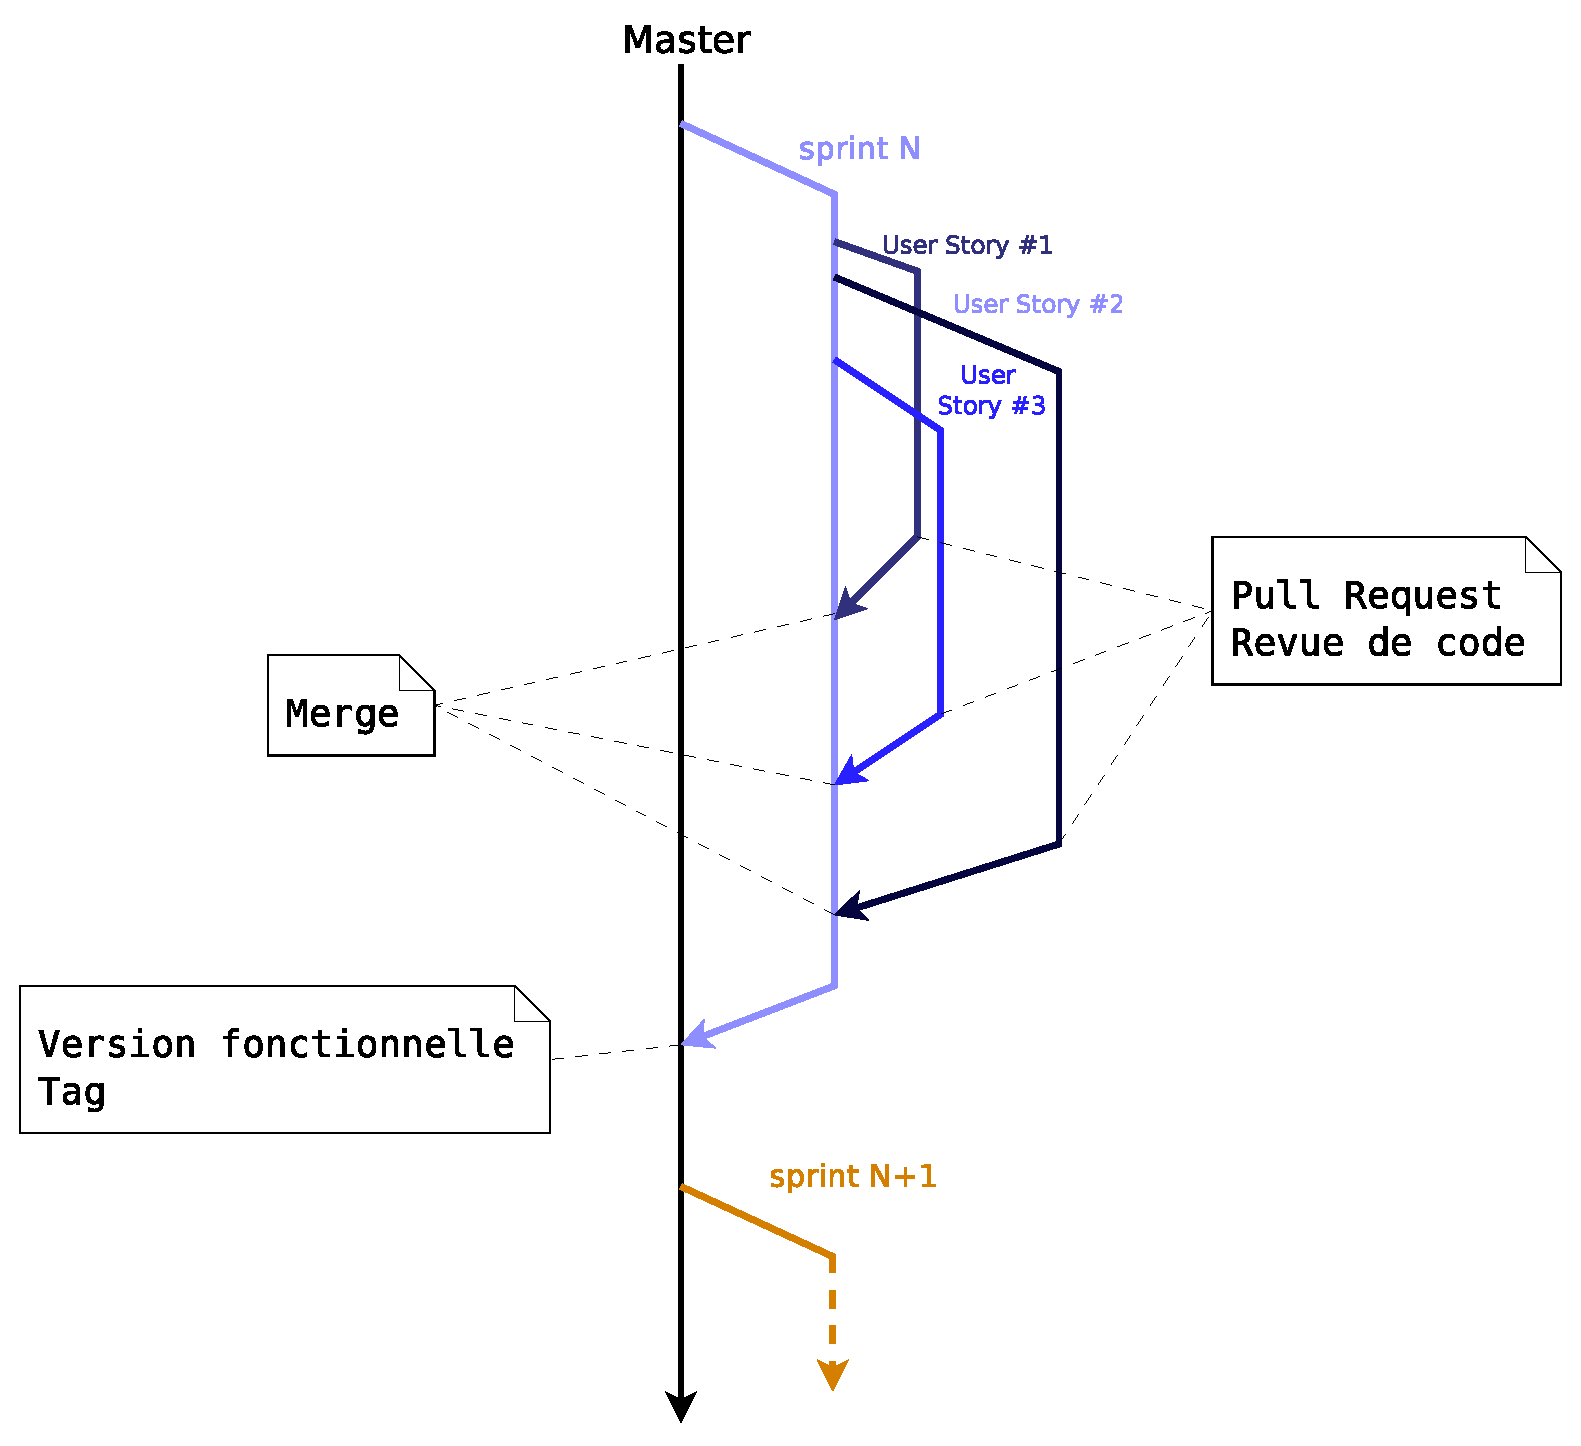
\includegraphics[width=0.83\linewidth]{images/Process/BranchingWorkflow}
	\caption{Git \textit{feature branch workflow}}
	\label{fig:BranchingWorkflow}
\end{figure}
\end{frame}
\begin{frame}{\ldots Continue}	
	\vfill
	Utilisation de \texttt{Travis-CI} : 
\begin{itemize}
	\item Tâches exécutées à chaque \textit{push} :
		\begin{itemize}
			\item Compilation du projet
			\item Exécution des tests unitaires
			\item Exécution des tests d'intégration
			\item Calcul de la couverture de code
			\item Déploiement de master sur Heroku
		\end{itemize}
\end{itemize}
\vfill
\centering
$\Longrightarrow$ Si tout est bon 
\includegraphics[width=1.2cm]{images/build}
\end{frame}
\ZacSpeak
\subsection{Vérification}
\begin{frame}{Vérification}
	\begin{itemize}
		\item Tests unitaires avec \texttt{Spock} pour : 
		\begin{itemize}
			\item Les classes de modèles
			\item Les contrôleurs
			\item Les services (hors DAO)
		\end{itemize}
		\vfill
		\item Calcul du taux de couverture avec \texttt{Cobertura} 
		\begin{itemize}
			\item Objectif de 80\% par ligne de code
		\end{itemize}
				\vfill
		\item Tableau de bord du projet à l'aide de \texttt{SonarQube}
		\begin{itemize}
			\item Couverture, documentation, commentaires, \ldots 
			\item Complexité de code
		\end{itemize}
				\vfill
		\item \texttt{Codenarc} pour l'analyse statique 
		\begin{itemize}
			\item Convention de codage standard Groovy
		\end{itemize}
	\end{itemize}
\end{frame}

\SteveSpeak
\subsection{Validation}
\begin{frame}{Validation}
		\begin{wrapfigure}{r}{6cm}
			\vspace{-60px}
			\centering
			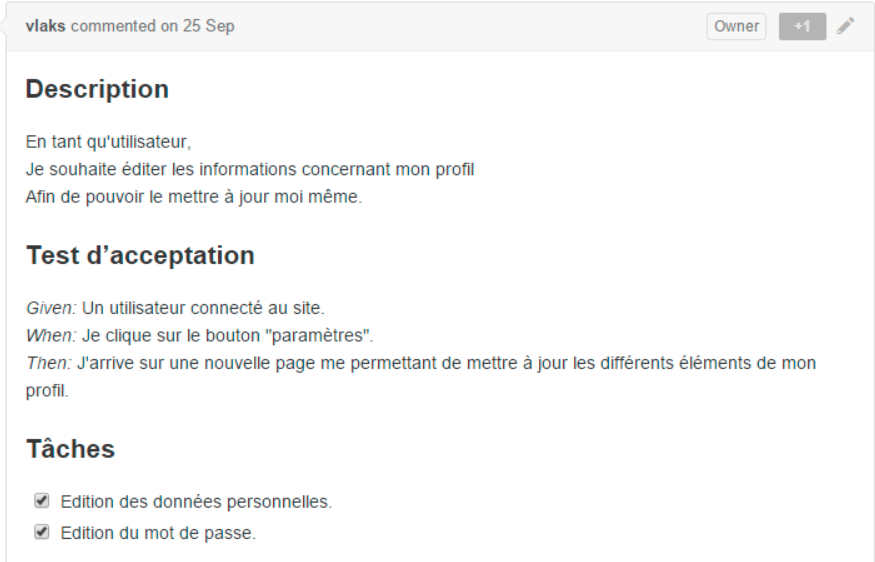
\includegraphics[width=6.3cm]{images/Process/accept-tests.png}
			\caption{\scriptsize Exemple de test d'acceptation}
			\label{fig:accept-tests}
		\end{wrapfigure}	
		\begin{minipage}{5cm}
			\begin{textblock}{6}(2.75,7)
			\begin{itemize}
				\item Tests d'intégration
				\item Tests d'acceptation
			\end{itemize}
			\end{textblock}
		\end{minipage}
\end{frame}


%\subsection{Qualification}
%\begin{frame}{Qualification}
%	\begin{itemize}
%		\item Déploiement continue de la branche master sur Heroku
%	\end{itemize}
%\end{frame}


	\section{Résultats} % Résultats = 5'
	
\subsection{Méthodologie}
\DylanSpeak
\begin{frame}{Résultats méthodologiques}
	\begin{itemize}
	\item Réalisation des \textit{issues} \scriptsize{(- de 10\% d’issues encore ouvertes)}
	\normalsize
	\item Principales fonctionnalités implémentées
	\item Mise en place de \textit{Scrum} \scriptsize{(revues et rétrospectives)}
	\end{itemize}
	\begin{figure}[H]
		\centering
		\includegraphics[width=0.8\linewidth]{"images/Results/methodo/badges"}
		\caption{\textit{Badges} du projet BandStorm}
		\label{fig:badges}
	\end{figure}\end{frame}
\SteveSpeak
\begin{frame}{Mise en place de SonarQube}
\begin{figure}
	\centering
	\includegraphics[width=0.95\linewidth]{"images/Results/methodo/sonar"}
	\caption{Tableau de bord de \texttt{SonarQube}}
	\label{fig:sonar}
\end{figure}
	
\end{frame}

\begin{frame}{Mise en place de Scrum}
	
\begin{figure}
\centering
\includegraphics[width=0.95\linewidth]{"images/Results/methodo/burndown"}
\caption{\textit{Burn-down chart} du Sprint 1}
\label{fig:burndown}
\end{figure}

\end{frame}

\ZacSpeak
\subsection{Produit}
\begin{frame}
\only<1>{
\begin{figure}
\centering
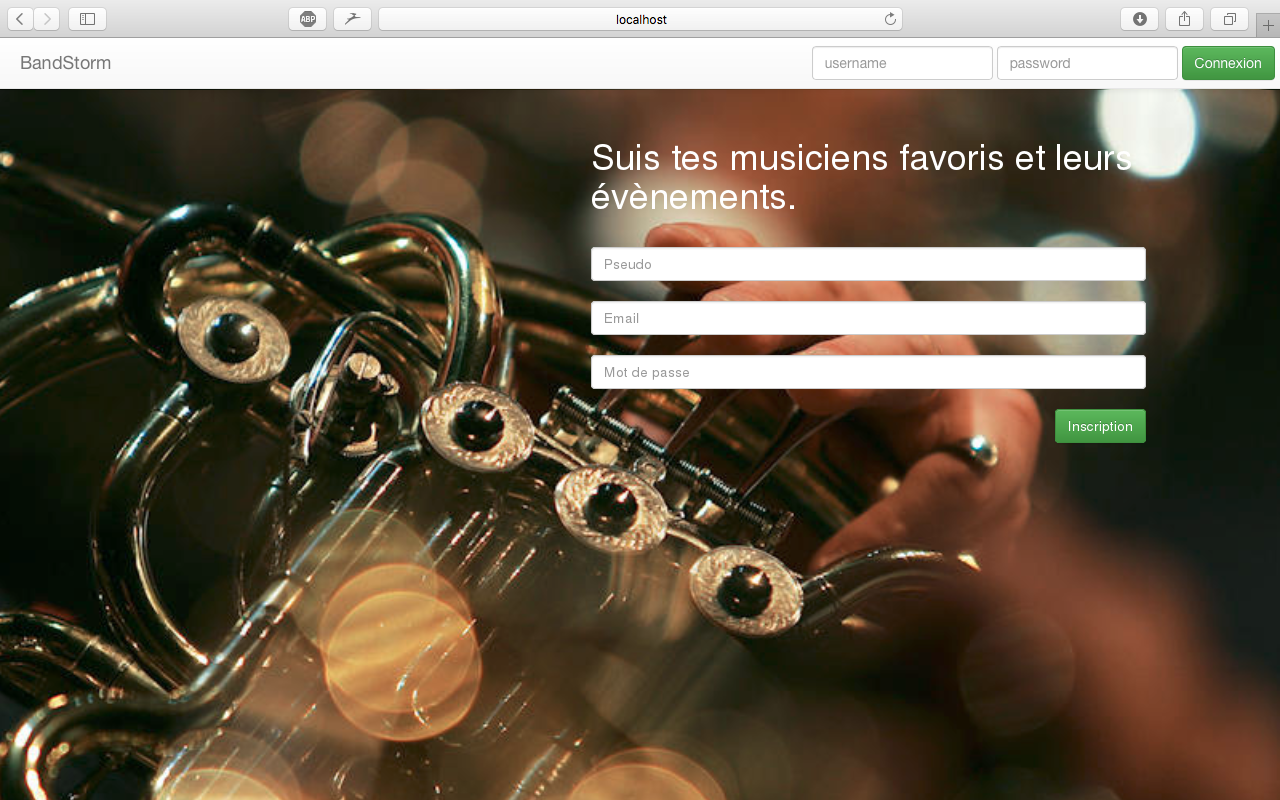
\includegraphics[width=0.95\linewidth]{images/Results/product/scshot1}
\caption{Page d'accueil des visiteurs}
\label{fig:scshot1}
\end{figure}
}
\only<2>{
\begin{figure}
\centering
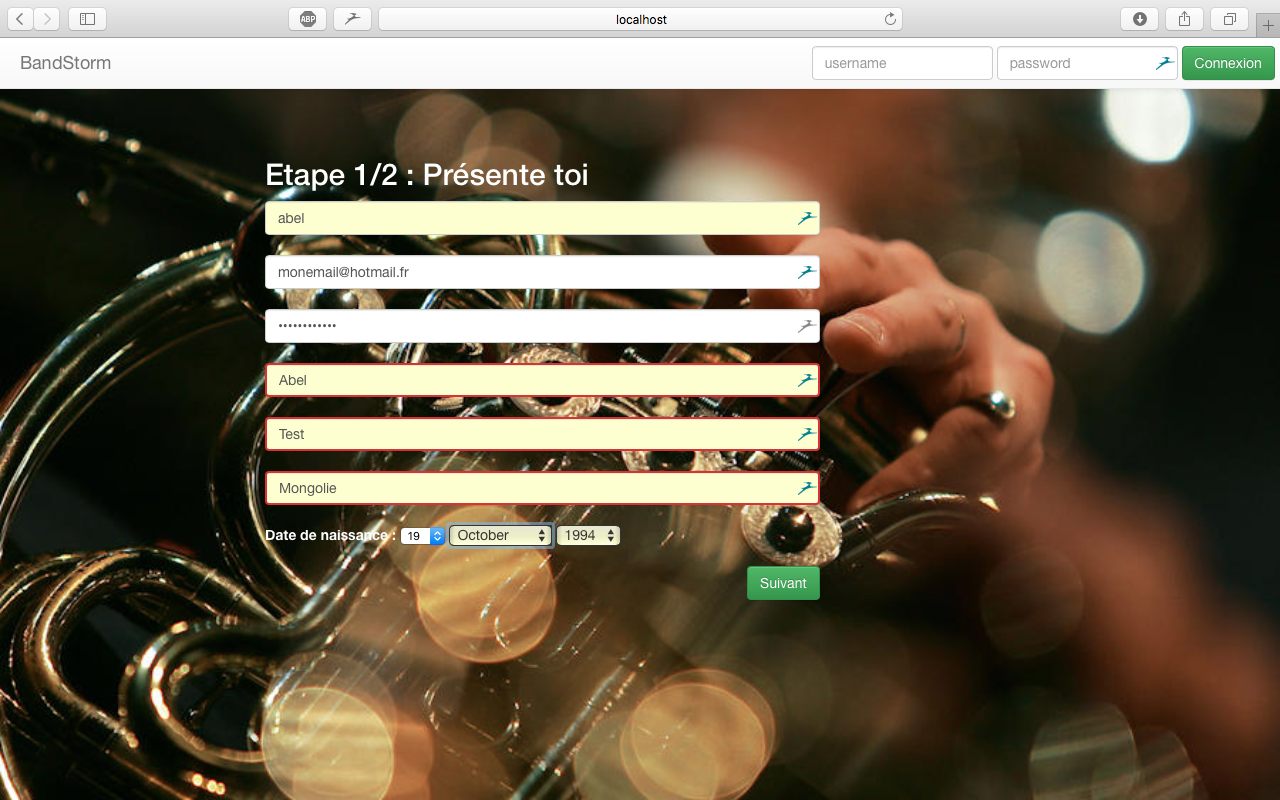
\includegraphics[width=0.95\linewidth]{images/Results/product/scshot2}
\caption{Inscription}
\label{fig:scshot2}
\end{figure}
}

\only<3>{
\begin{figure}
\centering
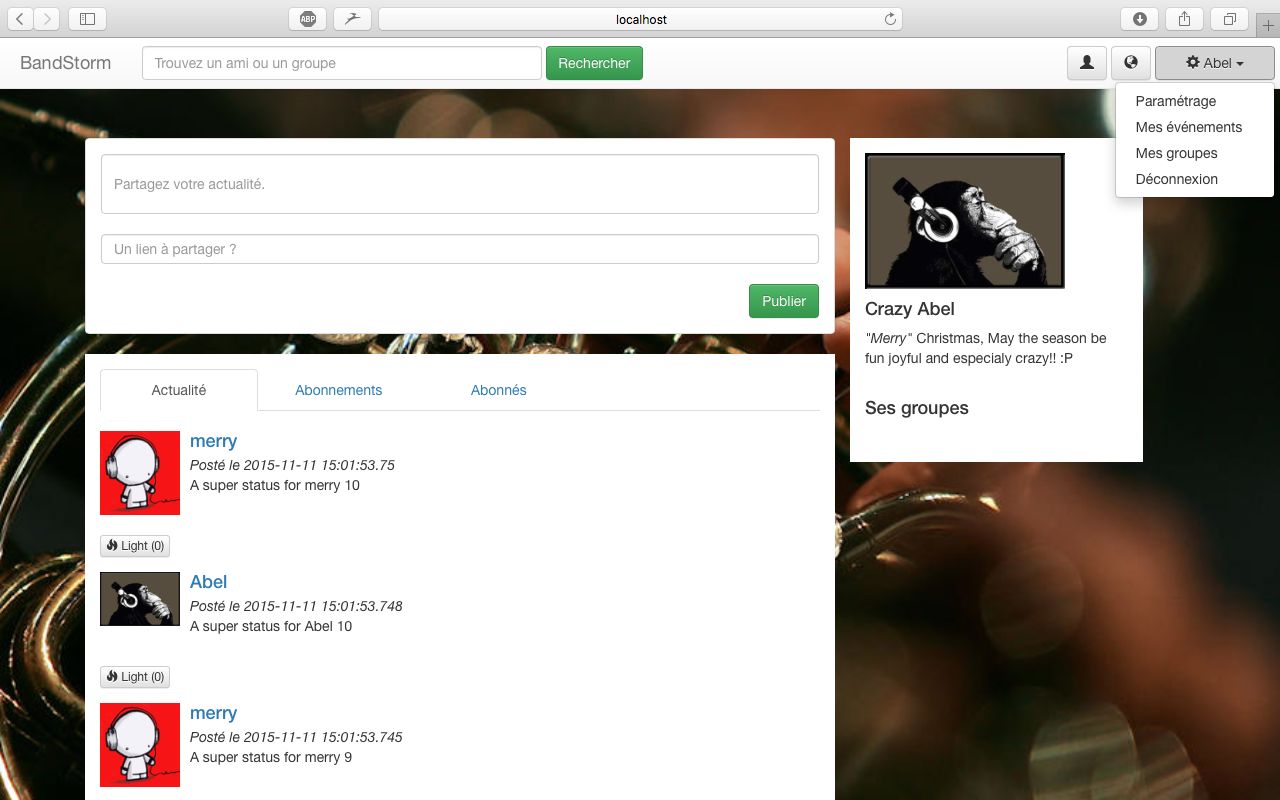
\includegraphics[width=0.95\linewidth]{images/Results/product/scshot4}
\caption{Page d'accueil des membres}
\label{fig:scshot4}
\end{figure}
}
\only<4>{
\begin{figure}
\centering
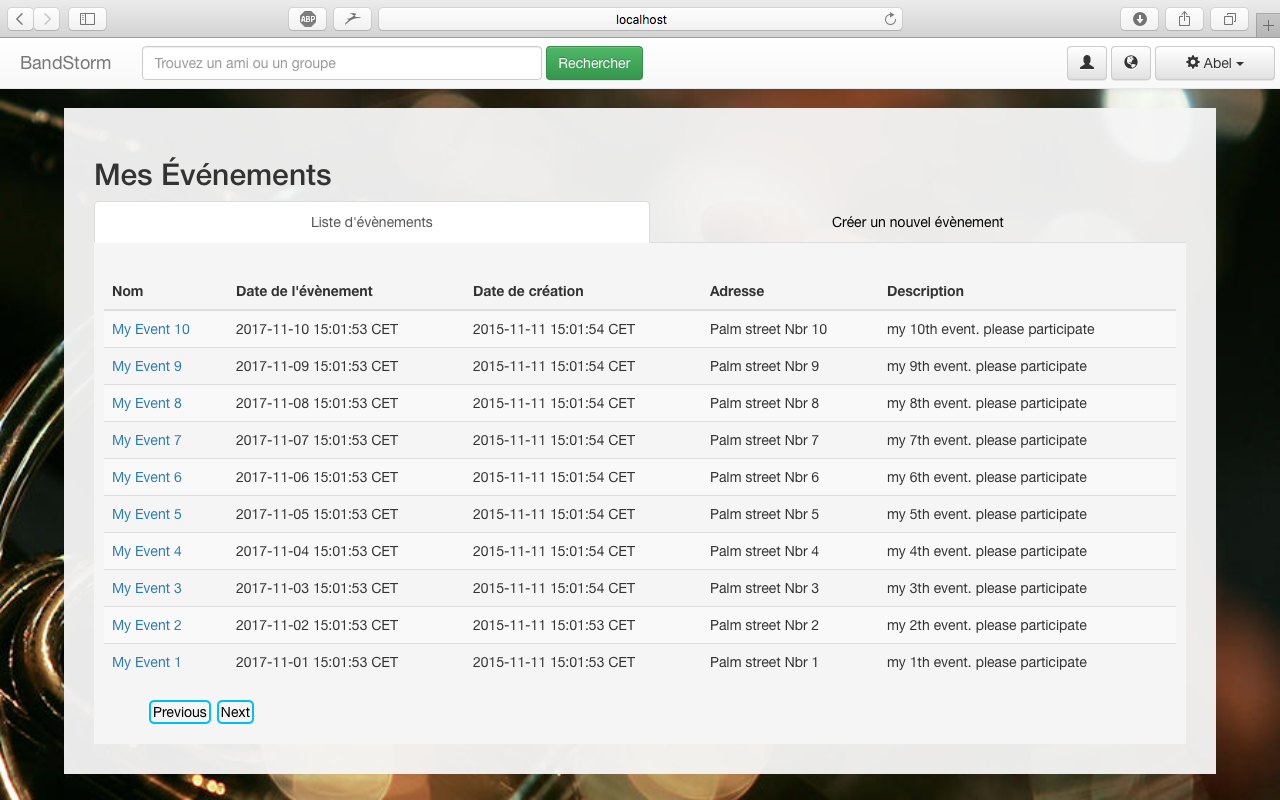
\includegraphics[width=0.95\linewidth]{images/Results/product/scshot5}
\caption{Liste des événements}
\label{fig:scshot5}
\end{figure}
}
\only<5>{
\begin{figure}
\centering
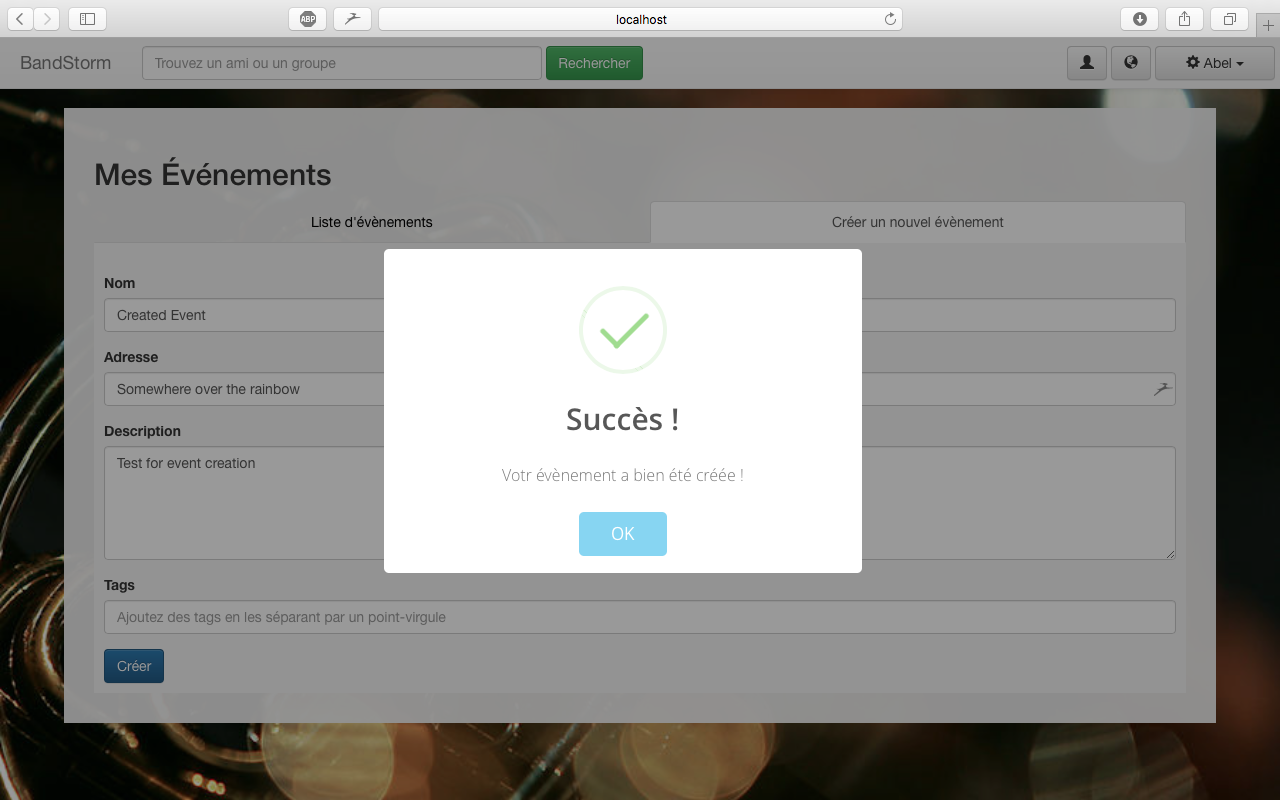
\includegraphics[width=0.95\linewidth]{images/Results/product/scshot6}
\caption{Création d'un événement}
\label{fig:scshot6}
\end{figure}
}
\only<6>{
\begin{figure}
\centering
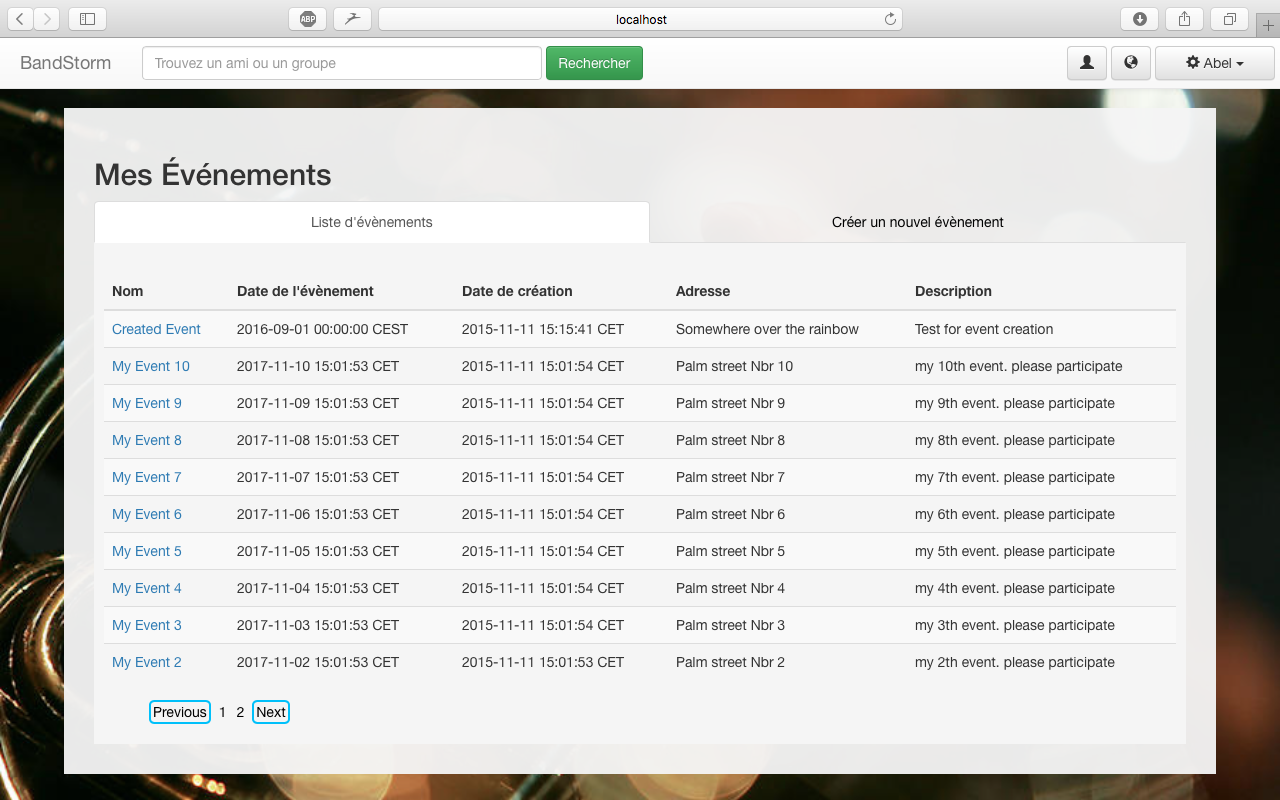
\includegraphics[width=0.95\linewidth]{images/Results/product/scshot7}
\caption{L'événement a été créé}
\label{fig:scshot7}
\end{figure}
}
\only<7>{
\begin{figure}
\centering
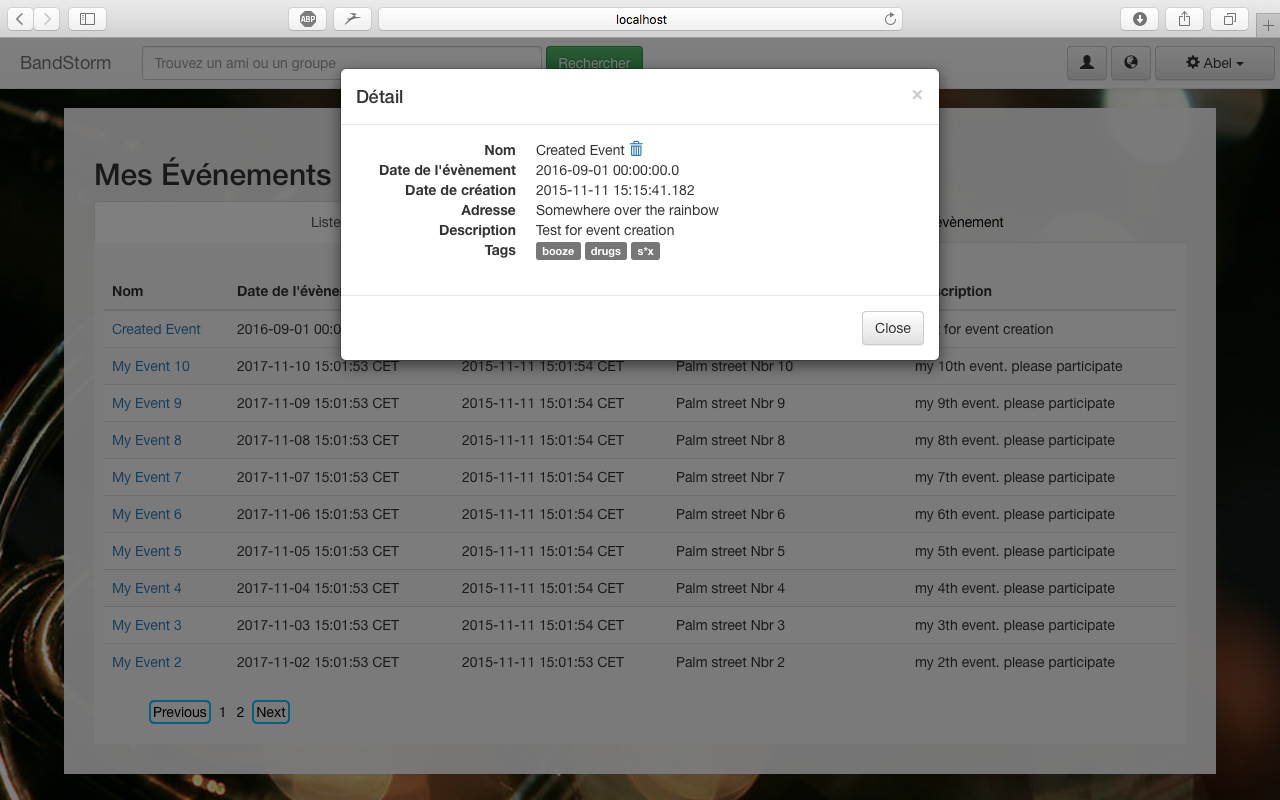
\includegraphics[width=0.95\linewidth]{images/Results/product/scshot8}
\caption{Détails de l'événement}
\label{fig:scshot8}
\end{figure}
}
\end{frame}



	\section{} % 3'
	\AntoineSpeak
\begin{frame}{Conclusion}
	\begin{alertblock}{De mauvais points\ldots}
		\begin{itemize}
			\item Mise en place de la méthode Scrum
			\item Reste des fonctionnalités à développer
		\end{itemize}
	\end{alertblock}
	\vfill
	\begin{exampleblock}{Mais beaucoup de positif !}
		\begin{itemize}
			\item Une application de qualité
			\item Expérience dans les méthodes Agiles
			\item Utilisation d'outils professionnels
			\begin{itemize}
				\item Travis-CI, Cobertura, SonarQube, \ldots
			\end{itemize}
		\end{itemize}
	\end{exampleblock}
\end{frame}


	% Slide for questions
	\sidetoc{no}
	\NooneSpeak{}
	\begin{frame}{Avez-vous des questions ?}
		\begin{figure}[H]
			\centering
	%		
\includegraphics[width=5cm]{interrogation.png}
		\end{figure}
	\end{frame}
	\vspace*{-7mm}    
	\begin{frame}[plain]{Product Backlog}
		\hspace*{-35mm}
	%	\includegraphics[width=13.8cm]{backlog.pdf}
	\end{frame}
	\begin{frame}
		\titlepage
	\end{frame}
\end{document}
